\documentclass[tikz,border=5pt]{standalone}
\usepackage{tikz}

\begin{document}
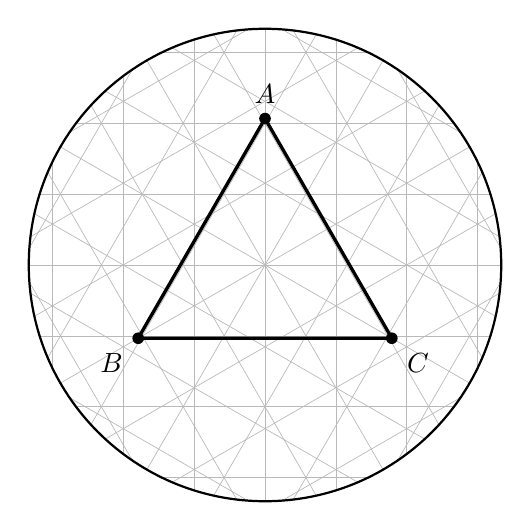
\begin{tikzpicture}[scale=3, line cap=round, line join=round]

  % Styles
  \tikzset{
    grid/.style={line width=0.25pt, gray!55},
    tri/.style={very thick}
  }

  % --- Geodesic grid (straight lines) behind ---
  \begin{scope}
    \clip (0,0) circle (1);

    % Helper: draw line with normal angle phi and offset c: n�x = c
    \newcommand{\DrawLine}[2]{%
      \pgfmathsetmacro{\phi}{#1}
      \pgfmathsetmacro{\c}{#2}
      \pgfmathsetmacro{\nx}{cos(\phi)} \pgfmathsetmacro{\ny}{sin(\phi)}
      \pgfmathsetmacro{\tx}{-sin(\phi)} \pgfmathsetmacro{\ty}{cos(\phi)}
      \pgfmathsetmacro{\root}{sqrt(max(0,1-\c*\c))}
      \pgfmathsetmacro{\cx}{\c*\nx} \pgfmathsetmacro{\cy}{\c*\ny}
      % Exact chord endpoints where the line meets the unit circle
      \draw[grid] ({\cx - \root*\tx},{\cy - \root*\ty}) --
                  ({\cx + \root*\tx},{\cy + \root*\ty});
    }

    % Six directions (every 30� up to 150�), several offsets
    \foreach \phi in {0,30,60,90,120,150}{
      \foreach \c in {-0.9,-0.6,-0.3,0,0.3,0.6,0.9}{
        \DrawLine{\phi}{\c}
      }
    }
  \end{scope}

  % Circular window (for visual consistency with the other models)
  \draw[thick] (0,0) circle (1);

  % --- Symmetric equilateral triangle ---
  \pgfmathsetmacro{\r}{0.62}
  \pgfmathsetmacro{\aA}{ 90}
  \pgfmathsetmacro{\aB}{210}
  \pgfmathsetmacro{\aC}{330}
  \pgfmathsetmacro{\Ax}{\r*cos(\aA)} \pgfmathsetmacro{\Ay}{\r*sin(\aA)}
  \pgfmathsetmacro{\Bx}{\r*cos(\aB)} \pgfmathsetmacro{\By}{\r*sin(\aB)}
  \pgfmathsetmacro{\Cx}{\r*cos(\aC)} \pgfmathsetmacro{\Cy}{\r*sin(\aC)}

  \draw[tri] (\Ax,\Ay) -- (\Bx,\By) -- (\Cx,\Cy) -- cycle;

  % Vertices
  \fill (\Ax,\Ay) circle (0.7pt) node[above=2pt] {$A$};
  \fill (\Bx,\By) circle (0.7pt) node[below left=2pt] {$B$};
  \fill (\Cx,\Cy) circle (0.7pt) node[below right=2pt] {$C$};

\end{tikzpicture}
\end{document}
